\documentclass[12pt, francais]{beamer}
%\usepackage[size=a4,scale=0.7,debug]{beamerposter}
\usepackage[francais]{babel}
\usepackage[utf8]{inputenc}
\usepackage[T1]{fontenc}

\usepackage{amsmath,amsfonts,amssymb}

\usepackage{booktabs}                   % just makes the table prettier
\usepackage{listings}                   % allow to include source code

\usepackage{color}                      % Enable color using
\usepackage{graphicx}     		     	% More option in included images
\usepackage{colortbl}
\usepackage{xcolor}



\DeclareGraphicsRule{*}{mps}{*}{}

\usetheme{minimal}
\usecolortheme{bam}
\setbeamertemplate{navigation symbols}{}


\title{Retour D'experience sur Symfony}
\date{}
\author{Djambazian Nicolas}
\logo{
\includegraphics[width=0.1\linewidth]{Pictures/logo.png}}


\lstset{
	basicstyle=\tiny,
	otherkeywords={public, function, private, class, return, extends, implements},
	keywordstyle=\color{bamred},
	stringstyle=\color{bamyellow},
	identifierstyle=\color{bamblue},
	commentstyle=\color{gray},
	breaklines=true
}


\begin{document}


\maketitle

\section{Qu'est-ce que Symfony ?}

\begin{frame}
	\catchline{C'est du PHP}
	\pause
	\begin{columns}
		\column[c]{.4\linewidth}
			\begin{block}{Mois}
				\begin{itemize}
					\centering
					\item  Vieux \\
					\item Pas de deamon \\
					\item Verbeux \\
				\end{itemize}
			\end{block}
		\column[c]{.4\linewidth}
			\begin{block}{Plus}
				\begin{itemize}
					\centering
					\item Vieux \\
					\item Orient\'e Objet \\
					\item Non typ\'e \\
					\item Reflection \\
					\item Namespace + Autoload \\
				\end{itemize}
			\end{block}
	\end{columns}
\end{frame}


\begin{frame}
	\catchline{Symfony, c'est des tas de trucs}
	\pause
	\begin{block}{}
		\begin{columns}
			\column[c]{.5\linewidth}
				\begin{itemize}
					\item MVC  \\
					\item Services avec injection de d\'ependances  \\
					\item Event Listener  \\
					\item Un gestionnaire de packet (composer)  \\
					\item Une tonne de Bundle  \\
				\end{itemize}
			\column[c]{.5\linewidth}
				\begin{itemize}
					\item ORM puissant \\
					\item Syst\`eme de routing \\
					\item Oganisation en Bundles \\
					\item Des tests fonctionnels (et unitaires) \\
					\item Des tas de Design pattern  \\
				\end{itemize}
		\end{columns}
	\end{block}
\end{frame}

\begin{frame}
	\catchline{Tout ce qui faut pour faire du code propre}
\end{frame}

\begin{frame}
	\catchline{Sans obligation bien sur}
	\lstinputlisting[language=PHP]{uglyCode.php}
	\pause
	\vspace*{-6cm}
	\begin{center}
		
\includegraphics[width=.5\linewidth]{Pictures/OhCrap.png}
	\end{center}
\end{frame}


\section{Une Api Rest en Symfony}

\begin{frame}
	\catchline{Pas (encore ?) de g\'en\'eration automatique}
\end{frame}


\begin{frame}
	\catchline{Des Bundles, encore des bundles}
	\begin{itemize}
	\centering
		\item FosRestBundle
		\item ApiDocBundle
		\item JMSSerializerBudle
	\end{itemize}
\end{frame}

\begin{frame}{FosRestBundle}
	\lstinputlisting[language=PHP]{fosrest.php}
\end{frame}


\begin{frame}{ApiDocBundle}
	\lstinputlisting[language=PHP]{apidoc.php}
\end{frame}

\begin{frame}{ApiDocBundle}
	\begin{center}
		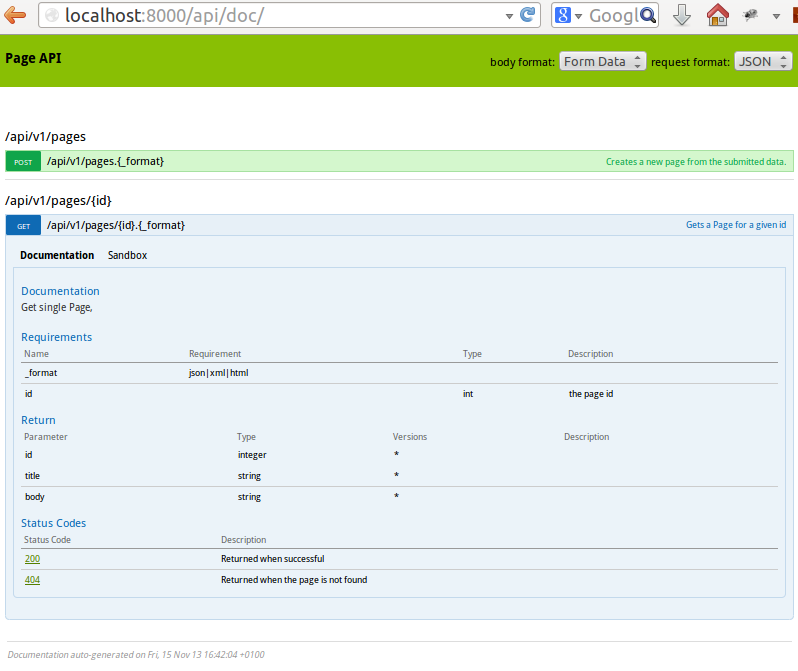
\includegraphics[width=.8\linewidth]{Pictures/apidoc.png}
	\end{center}

\end{frame}

\begin{frame}{JMSSerializerBudle}
	\lstinputlisting[language=PHP]{serializer.php}
\end{frame}


\begin{frame}
	\catchline{Et enfin, les formulaires Symfony}
	\lstinputlisting[language=PHP]{form.php}
	\lstinputlisting[language=PHP]{formsave.php}
\end{frame}


\begin{frame}
	\catchline{Magique !}
	\pause
	\catchline{Mais pas trop fait pour de l'API}
\end{frame}


\section{Bilan}



\begin{frame}
	\catchline{Lourd ! Mais puissant, bien architectur\'e, scalable, complet, ...}
\end{frame}
\begin{frame}
	\catchline{Ma Reco : Pour les gros projet}
\end{frame}




\end{document}
